%% thesis.tex 2014/04/11
%
% Based on sample files of unknown authorship.
%
% The Current Maintainer of this work is Paul Vojta.

\documentclass{ucbthesis}

\usepackage[american]{babel}
\usepackage{csquotes}
\usepackage[backend=biber, style=apa]{biblatex}
\DeclareLanguageMapping{american}{american-apa}
\bibliography{../../Documents/References/references.bib}

\usepackage{amsmath}


% To compile this file, run "latex thesis", then "biber thesis"
% (or "bibtex thesis", if the output from latex asks for that instead),
% and then "latex thesis" (without the quotes in each case).

% Double spacing, if you want it.  Do not use for the final copy.
% \def\dsp{\def\baselinestretch{2.0}\large\normalsize}
% \dsp

% If the Grad. Division insists that the first paragraph of a section
% be indented (like the others), then include this line:
% \usepackage{indentfirst}

\newtheorem{theorem}{Jibberish}

\hyphenation{mar-gin-al-ia}
\hyphenation{bra-va-do}

\begin{document}

% Declarations for Front Matter

\title{Bayesian and frequentist cross-validation methods for clustered and cross-clustered data}
\author{Daniel C. Furr}
\degreesemester{Spring}
\degreeyear{1995}
\degree{Doctor of Philosophy}
\chair{Professor Sophia Rabe-Hesketh}
\othermembers{Professor Alan Hubbard \\
              Assistant Professor Zacahary Pardos}
\numberofmembers{3}
\field{Education}
\campus{Berkeley}


\maketitle
% Delete (or comment out) the \approvalpage line for the final version.
\approvalpage
\copyrightpage

\begin{abstract}

% The text of the abstract goes here.  If you need to use a \section
% command you will need to use \section*, \subsection*, etc. so that
% you don't get any numbering.  You probably won't be using any of
% these commands in the abstract anyway.

The chapters of this dissertation are intended to be three independent, publishable papers, but they nevertheless share the theme of predictive inferences for explanatory item models.
Chapter 1 describes the differences between the Bayesian and frequentist statistical frameworks in the context of explanatory item response models. The particular model of focus, the ``doubly explanatory model'', is a model for dichotomous item responses that includes covariates for person ability and covariates for item difficulty. It includes many Rasch-family models as special cases. Differences in how the model is understood and specified within the two frameworks are discussed. The various predictive inferences available from the model are defined for the two frameworks. 

Chapter 2 is situated in the frequentist framework and focuses on approaches for explaining or predicting the difficulties of items. Within the frequentist framework, the linear logistic test model (LLTM) is likely to be used for this purpose, which in essence regresses item difficulty on covariates for characteristics of the items. However, this regression does not include an error term, and so the model is in general misspecified. Meanwhile, adding an error term to the LLTM makes maximum likelihood estimation infeasible. To address this problem, a two-stage modeling strategy (LLTM-E2S) is proposed: in the first stage Rasch model maximum likelihood estimates for item difficulties and standard errors are obtained, and in the second stage a random effects meta-analysis regression of the Rasch difficulties on covariates is performed that incorporates the uncertainty in the item difficulty estimates.
In addition, holdout validation, cross-validation, and Akaike information criteria (AIC) are discussed as means of comparing models that have different sets of item predictors.
I argue that AIC used with the LLTM estimates the expected deviance of the fitted model when applied to new observations from the \emph{same} sample of items and persons, which is unsuitable for assessing the ability of the model to predict item difficulties.
On the other hand, AIC applied to the LLTM-E2S provides the expected deviance related to new observations arising from \emph{new} items, which is what is needed.
A simulation study compares parameter recovery and model comparison results for the two modeling strategies.

Chapter 3 takes a Bayesian outlook and focuses on models that explain or predict person abilities. I argue that the usual application of Bayesian forms of information criteria to these models yields the wrong inference.
Specifically, when using likelihoods that are conditional on person ability, information criteria estimate the expected fit of the model to new data arising from the \emph{same} persons.
What are needed are likelihoods that are marginal over the distribution for ability, which may be used with information criteria to estimate the expected fit to new data from a \emph{new} sample of persons. 
The widely applicable information criterion (WAIC), Pareto-smoothed importance sampling approximation to leave-one-out cross-validation, and deviance information criterion (DIC) are discussed in the context of these conditional and marginal likelihoods. 
An adaptive quadrature scheme for use within Markov chain Monte Carlo estimation is proposed to obtain the marginal likelihoods.
Also, the moving block bootstrap is investigated as a means to estimate the Monte Carlo error for Bayesian information criteria estimates. 
A simulation study using a linear random intercept model is conducted to assess the accuracy of the adaptive quadrature scheme and the bootstrap estimates of Monte Carlo error.
These methods are then applied to an real item response dataset, demonstrating the practical difference between conditional and marginal forms of information criteria.

\end{abstract}


\begin{frontmatter}

\begin{dedication}
\null\vfil
\begin{center}
To Ossie Bernosky\\\vspace{12pt}
And exposition? Of go. No upstairs do fingering. Or obstructive, or purposeful.
In the glitter. For so talented. Which is confines cocoa accomplished.
Masterpiece as devoted. My primal the narcotic. For cine? To by recollection
bleeding. That calf are infant. In clause. Be a popularly. A as midnight
transcript alike. Washable an acre. To canned, silence in foreign.
\end{center}
\vfil\null
\end{dedication}

% You can delete the \clearpage lines if you don't want these to start on
% separate pages.

\tableofcontents
\clearpage
\listoffigures
\clearpage
\listoftables

\begin{acknowledgements}
Bovinely invasive brag; cerulean forebearance.
Washable an acre. To canned, silence in foreign.
Be a popularly. A as midnight transcript alike.
To by recollection bleeding. That calf are infant. In clause.
Buckaroo loquaciousness?  Aristotelian!
Masterpiece as devoted. My primal the narcotic. For cine?
In the glitter. For so talented. Which is confines cocoa accomplished.
Or obstructive, or purposeful.
And exposition? Of go. No upstairs do fingering.

\end{acknowledgements}

\end{frontmatter}

\pagestyle{headings}

% (Optional) \part{First Part}

\newpage
\chapter{Cross-validation for cross-clustered data}
\documentclass[12pt, letterpaper]{article}
\usepackage[left=1.00in, right=1.00in, top=1.00in, bottom=1.00in]{geometry}
\usepackage{tikz} \usetikzlibrary{arrows.meta}
\usepackage{caption}
\usepackage{subcaption}
\usepackage{amsmath}

\usepackage[american]{babel}
\usepackage{csquotes}
\usepackage[backend=biber, style=apa]{biblatex}
\DeclareLanguageMapping{american}{american-apa}
\bibliography{../../../Documents/References/references.bib}

\title{A comparison of the frequentist and Bayesian frameworks in relation to explanatory item response models}
\author{Daniel Furr}
\date{\today}


\begin{document}

% Tikz styles presets ----------------------------------------------------------

% Parameter and data nodes
\tikzstyle{p} = [circle, draw=black, fill=blue!10, thick,
                 inner sep=1pt, minimum size=8mm]
\tikzstyle{d} = [rectangle, draw=black, fill=blue!10, thick,
                 inner sep=1pt, minimum size=8mm]

% Replicate parameter and data nodes
\tikzstyle{pr} = [circle, draw=gray, fill=white, thick,
                  inner sep=1pt, minimum size=8mm]
\tikzstyle{dr} = [rectangle, draw=gray, fill=white, thick,
                  inner sep=1pt, minimum size=8mm]

% Arrow styles for model specification and for generating quantities
\tikzstyle{marrow} = [solid, -{Stealth[length=2mm]}, draw=black]
\tikzstyle{garrow} = [solid, -{Stealth[length=2mm]}, draw=gray]


% Invisisble node (for maintaining equal figure sizes_
\tikzstyle{i} = [circle, draw=none, fill=none, text=white]

% Box for PPCM part of model
\tikzstyle{ppmc}=[fill=red!10, draw=white]

% Boxes and labels to indicate clustering in models
\tikzstyle{items-box}    = [fill = none, draw = black!30!green]
\tikzstyle{items-node}   = [text = black!30!green, anchor = south east]
\tikzstyle{persons-box}  = [fill = none, draw = black!20!orange]
\tikzstyle{persons-node} = [text = black!20!orange, anchor = north west]

\maketitle

\newcommand{\iiiiint}{\int \!\!\! \int \!\!\! \int \!\!\! \int \!\!\! \int}
\newcommand{\iiiiiint}{\int \!\!\! \int \!\!\! \int \!\!\! \int \!\!\! \int \!\!\! \int}


\section{Introduction}

Item response data are cross-classified; that is, any given response to an item is nested both within a person and within an item.
In developing a model for such data, either or both of persons and items may be regarded as arising from a distribution, and the mean of these distributions may be conditional on characteristics of persons or items.
In this way, an item response model may be described as explanatory if it estimates the effects of person or item characteristics on the abilities of people or the difficulties of items.

Rasch-family item response models are the focus of this chapter. In the frequentist framework, some explanatory Rasch-family models cannot be estimated using the usual marginal maximum likelihood estimation.
In particular, marginal maximum likelihood estimation is infeasible if both the persons and items are modeled as arising from distributions.
However, when persons but not items are assumed to arise from a distribution, a variety of standard software packages are available to fit such models with relative ease.
There is no such barrier in the Bayesian framework, as models for cross-classified data may be estimated using Markov chain Monte Carlo (MCMC) simulation. The existing software for MCMC tends to be highly flexible but more cumbersome to use.

In this chapter, frequentist and Bayesian approaches to explanatory item response modeling are compared.
Special attention is paid to the predictive inferences that are available under the two frameworks.
Despite the particular context of item response models, the discussion applies to models for clustered data more generally.


\section{A doubly explanatory item response model}

\subsection{General formulation}

A useful model for dichotomous item response data is the Rasch model \parencite{Rasch1960a}:
\begin{equation} \label{eq:base}
	\Pr ( y_{ip} | \theta_p, \delta_i) =
	\frac {\exp(\theta_p - \delta_i)^{y_{ip}}}
	{1 + \exp(\theta_p - \delta_i)}
,\end{equation}
where $y_{ip} = 1$ if person $p$ ($p = 1, \dotsc, P$) responded to item $i$ ($i = 1, \dotsc, I$) correctly and $y_{ip} = 0$ otherwise, $\theta_p$ is the ability parameter for person $p$, and $\delta_i$ is the difficulty parameter for item $i$. The individual instances of $\theta_p$ and $\delta_i$ may be collected into vectors $\theta$ and $\delta$, respectively. This is a ``descriptive'' item response model \parencite{Wilson2004}; it fully accounts for abilities and difficulties, assuming the appropriateness of the model, but does not offer insight into the factors associated with abilities and difficulties.

The model in Equation~\ref{eq:base} may be expanded to a ``person explanatory'' model by decomposing $\theta_p$ as
\begin{equation} \label{eq:theta}
	\theta_p = w_p' \gamma + \zeta_p
,\end{equation}
where $w_p$ is a row from a design matrix $W$ for person-related covariates, $\gamma$ is a vector of regression parameters, and $\zeta_p$ is the residual person ability. The above may be interpreted as a latent regression of ability on covariates $w_p$. $\theta_p$ may be referred to as the composite ability, $w_p' \gamma$ the structured part of ability, and $\zeta_p$ the residual part.

Similarly, decomposing $\delta_i$ as
\begin{equation} \label{eq:delta}
	\delta_i = x_i' \beta + \epsilon_i
\end{equation}
results in an ``item explanatory'' model, in which $x_i$ is a row from a design matrix $X$ for item-related covariates, $\beta$ is a vector of regression parameters, and $\epsilon_i$ is the residual item difficulty. The above is then a latent regression of item difficulty on covariates $x_i$. In parallel with the preceding terminology for ability, $\delta_i$ may be referred to as the composite difficulty, $x_i' \beta$ the structured part of difficulty, and $\epsilon_i$ the residual part.

Equations~\ref{eq:base}, \ref{eq:theta}, and \ref{eq:delta} together form a ``doubly explanatory'' item response model, which incorporates covariates associated with both the persons and items. Note that the model may still serve descriptive purpose as the composite abilities and difficulties remain a part of the model. The final step in formulating the model is to specify distributions for the residuals. In this chapter, normal distributions are assumed,
\begin{equation}
	\zeta_p \sim N(0, \sigma^2)
\end{equation}
and
\begin{equation}
	\epsilon_i \sim N(0, \tau^2)
,\end{equation}
though other choices could be considered. The person and item ``sides'' of the model are specified in directly parallel ways, and much of the discussion that follows will make use of this point.

The model is also presented as a directed graphical model \parencite[for example,][]{dawid1999probabilistic, jordan2004graphical} in Figure~\ref{fig:eirm-model}. In the diagram, parameters are represented by circles, and data are represented by squares. The boxed regions indicate whether the parameters vary over persons, items or neither, and naturally the item responses $y$ vary over both. The direction of the arrows indicates dependence. For example, $\theta$ depends on $\gamma$ and $\zeta$ directly, while it depends indirectly on $\sigma$.

\begin{figure}[btp]
	\centering
	\centering
\begin{tikzpicture}[scale=.75, transform shape]

  \node [p]  (z)  at (0,10) {$\zeta$};
  \node [p]  (s)  at (2,10) {$\sigma$};

  \node [p]  (o)  at (0, 8) {$\theta$};
  \node [p]  (c)  at (2, 8) {$\gamma$};

  \node [d]  (y)  at (0, 6) {$y$};

  \node [p]  (d)  at (0, 4) {$\delta$};

  \node [p]  (e)  at (0, 2) {$\epsilon$};
  \node [p]  (b)  at (2, 4) {$\beta$};
  
  \node [p]  (t)  at (2, 2) {$\tau$};

  \draw [items-box] (-1, 0.75) rectangle (1.25, 7);
  \node [items-node] at (1.25, 0.75) {Items $i$};
  
  \draw [persons-box] (-1.25, 11.25) rectangle (1.00, 5);
  \node [persons-node] at (-1.25, 11.25) {Persons $p$};

  \foreach \from/\to in {s/z, c/o, z/o, o/y, d/y, b/d, t/e, e/d}
    \draw [marrow] (\from) -- (\to);

\end{tikzpicture}
	\caption[The doubly explanatory model]
	{The doubly explanatory model presented as a directed graphical model. Circles represent parameters and squares represent data. Person covariates $w_p$ and item covariates $x_i$ are omitted. The boxed regions indicate whether the parameters vary over persons, items or neither.}
	\label{fig:eirm-model}
\end{figure}


\subsection{Hierarchical Bayes modeling approach}

In Bayesian methodology, the posterior distribution for the parameters is factorized by way of Bayes theorem:
\begin{equation} \label{eq:bayes}
	p(\omega | y, W, X) \propto
	p(\omega)
	p(y | \omega, W, X)
,\end{equation}
which indicates that the posterior distribution proportional to the product of the prior distribution and the likelihood. In the above, $\omega$ is the set of model parameters. In this chapter, the following terminology for different types of parameters is used.
\begin{enumerate}
	\item \emph{Basic parameters}
	are the foundational parameters. They are plugged into the likelihood directly or affect it indirectly through intermediate parameters. Priors are specified for them.
	\begin{enumerate}
		\item \emph{Exchangeable basic parameters}
		have hierarchical prior distributions. They are exchangeable draws from a distribution, the characteristics of which are determined by hyperparameters. Residuals $\zeta_p$ and $\epsilon_i$ are examples.
		\item \emph{Non-exchangeable basic parameters}
		have non-hierarchical priors. They are not thought of as exchangeable or drawn from a distribution, except in the loose sense that there is some prior distribution. Regression coefficients $\gamma$ and $\beta$ are examples.
	\end{enumerate}
	\item \emph{Intermediate parameters}
	are composites built from basic parameters. They may be included in Bayesian modeling to streamline specifying a model or they may be quantities of genuine interest. They may be plugged into the likelihood in place of basic parameters. They do not have explicit prior distributions, but instead their priors follow from the priors for the basic parameters. Parameters $\theta_p$ and $\delta_i$ are examples
	\item \emph{Hyperparameters}
	are parameters for the estimated distributions for exchangeable basic parameters. These are not plugged into the likelihood but rather determine the prior distributions for the exchangeable parameters. They do have prior distributions themselves.
\end{enumerate}
Of the above terms, only ``hyperparameters'' is in general usage, while the remaining types of parameters are not typically distinguished from one another.

The doubly descriptive model has a likelihood (Equation~\ref{eq:base}) based on intermediate parameters $\theta$ and $\delta$, which are in turn built from basic parameters $\gamma$, $\zeta$, $\delta$, and $\epsilon$ (Equations~\ref{eq:theta} and \ref{eq:delta}). $\gamma$ and $\delta$ are non-exchangeable basic parameters, while $\zeta$ and $\epsilon$ are exchangeable basic parameters whose priors depend on hyperparameters $\sigma$ and $\tau$, respectively.
The prior distribution in Equation~\ref{eq:bayes} may be rewritten as
\begin{equation} \label{eq:prior}
	p(\omega) =
	p(\gamma) p(\sigma)
	\left [
		\prod_{p=1}^P p(\zeta_p | \sigma)
	\right ]
	p(\beta) p(\tau)
	\left [
		\prod_{i=1}^I p(\epsilon_i | \tau)
	\right ]
\end{equation}
if independent priors are specified, which is the usual case. No prior is included for $\theta$ and $\delta$ as they are wholly determined from the basic parameters.
%The joint prior $p(\gamma, \beta, \tau, \sigma, \zeta, \epsilon)$ may be written as the product of individual priors if the priors are specified as independent, which is the usual case.
The likelihood part of Equation~\ref{eq:bayes} may be rewritten in terms of basic parameters as
\begin{equation} \label{eq:bayes-likelihood-alt}
	p(y | \omega, W, X) =
%	p(y | W, X, \gamma, \beta, \zeta, \epsilon) =
	\prod_{p=1}^P \prod_{i=1}^I
	\Pr(y_{ip} | w_p, x_i, \zeta_p, \gamma, \epsilon_i, \beta)
,\end{equation}
%where $\omega = \{\gamma, \beta, \sigma\}
or in terms of intermediate parameters as
\begin{equation} \label{eq:bayes-likelihood}
	p(y | \omega, W, X) =
	p(y | \theta, \delta) =
	\prod_{p=1}^P \prod_{i=1}^I \Pr(y_{ip} | \theta_p, \delta_i)
.\end{equation}
Given that both the prior and the likelihood may be specified ignoring the intermediate parameters $\theta$ and $\delta$, it is clear that they are redundant. For many applications, however, they have useful interpretations, and for that reason estimation of their posteriors may be desired. Further, the posterior distributions of $\theta$ and $\delta$ can be estimated easily from the posterior draws of the basic parameters.

The posterior for a single parameter, marginal in regards to all other parameters, may be obtain by integrating the full joint posterior over all other parameters. Let $D = \{ y, W, X \}$ represent the full data. Then,
\begin{equation}
	p(\sigma | D) =
	\iiiiint
		p(\zeta, \gamma, \sigma, \epsilon, \beta, \tau | D)
	~d \zeta d \gamma d \epsilon d \beta d \tau
\end{equation}
is the posterior for the standard deviation of the ability residuals. The mean and standard deviation of the marginal posterior for a parameter may be taken to represent a point estimate and standard error. Further, the joint posterior of a subset of parameters, $p(\beta, \zeta_p, \gamma, \epsilon_i | D)$ for example, likewise may be obtained by integrating out the other parameters. Despite the high-dimensional integral involved, these quantities are readily available from Monte Carlo simulation by simply ignoring the draws for the parameters to be integrated out, and so no special effort is required to obtain them.

The model could equivalently be specified using hierarchical centering \parencite{gelfand1995efficient} by replacing the preceding prior with
\begin{equation}
	p(\omega) =
	p(\gamma) p(\sigma)
	\left [
		\prod_{p=1}^P p(\theta_p | w_p, \gamma, \sigma)
	\right ]
	p(\beta) 	p(\tau)
	\left [
		\prod_{i=1}^I p(\delta_i | x_i, \beta, \tau)
	\right ]
\end{equation}
where
$p(\theta_p | w_p, \gamma, \sigma) = \mathrm{N}(w_p \gamma, \sigma^2)$ and
$p(\delta_i | x_i, \beta, \tau)    = \mathrm{N}(x_i \beta, \tau^2)$,
respectively. The likelihood is still specified as in Equation~\ref{eq:bayes-likelihood}. In this formulation, residuals $\zeta$ and $\epsilon$ are omitted altogether, and $\theta$ and $\delta$ are treated as exchangeable (conditional on covariates) basic parameters rather than as intermediate parameters. Depending on the data and on the algorithm used, this formulation may improve the efficiency of the MCMC simulation. Because this chapter includes discussion of inferences related to the residuals, the ``decentered'' formulation described before is preferred.


\subsection{Frequentist modeling approach}

In the frequentist approach, only the non-exchangeable basic parameters ($\gamma$ and  $\beta$) and the hyperparameters ($\sigma$ and $\tau$) are treated as parameters to be estimated. In this framework, marginal maximum likelihood may be used to estimate the model, which involves marginalizing the residuals out of the likelihood. The marginal likelihood is
\begin{equation} \label{eq:marginal-likelihood}
p(y | \gamma, \beta, \sigma, \tau) =
\int \cdots \iint \cdots \int
	\prod_{p=1}^P \prod_{i=1}^I
	\left [
		\Pr(y_{ip} | \zeta_p, \gamma, \epsilon_i, \beta)
		p(\zeta_p | \sigma)
		p(\epsilon_i | \tau)
	\right ]
~d \zeta_1 \ldots d \zeta_P d \epsilon_1 \ldots d \epsilon_I
,\end{equation}
in which the probability of a response is marginal over the distributions for person and item residuals. Point estimates $\hat\gamma$, $\hat\sigma$, $\hat\beta$, and $\hat\tau$ are obtained by maximizing this likelihood

Within this framework, the exchangeable parameters $\zeta$ and $\epsilon$ are called latent variables or random effects because parameters cannot have distributions. Rather than obtain direct estimates for random effects, marginal maximum likelihood estimation obtains estimates for the parameters of their distributions only, in this case, $\hat \sigma$ and $\hat\tau$. The non-exchangeable basic parameters $\gamma$ and $\beta$ are sometimes referred to as ``fixed-effects.''
%\emph{``Can choose whether to treat $\zeta_p$ or $\epsilon_i$ as latent variables (random effects) or just consider their marginal likelihood, for example, to just get a covariance structure.'' Ref: Molenberghs and Verbeke. Hard to find because they wrote a million articles together.}

A model of this kind may be formulated in the generalized linear mixed model framework. The response variable, conditional on covariates and so-called random effects, is specified as arising from a Bernoulli distribution:
\begin{equation}
	y_{ip} | w_p, x_i, \zeta_p, \epsilon_i \sim \mathrm{Bernoulli}(\pi_{ip})
.\end{equation}
Then the model may be written in terms of an inverse link function
\begin{equation}
	\pi_{ip} =
	\Pr(y_{ip} = 1 | w_p, x_i, \zeta_p, \epsilon_i) =
	\mathrm{logit}^{-1}[\eta_{ip}]
\end{equation}
and a linear predictor
\begin{equation}
	\eta_{ip} =
	(w_p'\gamma + \zeta_p) -
	(x_i'\beta + \epsilon_i)
.\end{equation}
Because the random-effects $\zeta_p$ and $\epsilon_i$ are not nested, the model may be described as a crossed-random effects model. Such a model is difficult to estimate efficiently via marginal maximum likelihood because the integrals in Equation~\ref{eq:marginal-likelihood} do not factorize as they do with nested random effects. The result is an $I \times P$ dimensional integral, though \textcite{rasbash1994efficient} describe a means of reducing this to an $I + 1$ dimensional integral.

%double integration over the latent distributions (see Equation~\ref{eq:mml-likelihood}). The Laplace approximation may be employed to make the math tractable, but this approach has known shortcomings \parencite{Joe2008}.

%Though not directly estimated, post-hoc estimates for $\hat\zeta_p$ and $\hat\epsilon_i$ may be obtained by finding the mean or mode of $p(\yp|\zeta_p) p(\zeta_p|\hat\sigma)$ or $p(\yi|\epsilon_i) p(\epsilon_i|\hat\tau)$, which are referred to as ``empirical Bayes'' estimates. Standard errors are available for these, though they are calculated as though the parameter estimates are known, rather than random, quantities.
%
%Also available only in post-analysis are estimates
%$\hat\theta_p = w_p' \hat\gamma + \hat\zeta_p$ and
%$\hat\delta_i = x_i' \hat\beta + \hat\epsilon_i$,
%where $\hat\zeta_p$ and $\hat\epsilon_i$ are empirical Bayes estimates. Standard errors are available for these quantities, though they also are calculated as if the parameter estimates are known quantities.


\subsection{Special cases}
\label{sec:special-cases}

Many dichotomous item response models are special cases of the doubly explanatory model that arise from restrictions placed on the composite abilities and difficulties. For example, the the Rasch model \parencite{Rasch1960a} as fit by marginal maximum likelihood estimation \parencite{bock1981marginal} can be written as
\begin{equation}
	\Pr ( y_{ip} | \theta_p, \delta_i) =
	\frac {\exp(\theta_p - \delta_i)^{y_{ip}}}
	{1 + \exp(\theta_p - \delta_i)}
\end{equation}
\begin{equation}
	\theta_p = \zeta_p
\end{equation}
\begin{equation}
	\delta_i = x_i' \beta
,\end{equation}
where $X$ is an $I \times I$ identity matrix ($I_I$) and $\beta$ is a vector of length $I$, such that $\delta_i = \beta_i$. In other words, $\delta_i$ is set equal to the (unstructured) structural part of item difficulty, while $\theta_p$ is set equal to the ability residuals.

In the Bayesian approach, the posterior for this Rasch model variant is given by
\begin{equation}
	p(\theta, \sigma, \delta | y) \propto
	\left [
		p(\delta) 	p(\sigma)
		\prod_{p=1}^P p(\theta_p | \sigma)
	\right ]
	\left [
		\prod_{p=1}^P \prod_{i=1}^I
		\Pr ( y_{ip} | \theta_p, \delta_i)
	\right ]
,\end{equation}
in which the left hand bracketed quantity is the prior and and the right hand quantity is the likelihood. The marginal likelihood for the frequentist approach is
\begin{equation}
	p(y | \sigma, \delta) =
	\prod_{p=1}^P
	\int
		\prod_{i=1}^I
		\Pr(y_{ip} | \theta_p, \delta_i)
		p(\theta_p | \sigma)
	~d \theta_p
.\end{equation}
The single dimensional integration is simpler than the $I \times P$ dimensional integral in Equation~\ref{eq:marginal-likelihood} and may be approximated using adaptive quadrature \parencite{rabe2002reliable}.

\begin{table}
	\centering
	\begin{tabular}{lccc}
		\hline
		Model	& $\theta_p$ & $\delta_i$ & Notes \\ \hline
		MML Rasch
			& $\zeta_p$ & $x_i'\beta$ & $X = I_I$ \\
		JML Rasch
			& $w_p' \gamma$ & $x_i'\beta$ & $W = I_{P-1}$, $X = I_I$ \\
		Random item Rasch
			& $\zeta_p$ & $\epsilon_i$ &  \\
		Latent regression
			& $w_p' \gamma + \zeta_p$ & $x_i'\beta$ & $X = I_I$ \\
		Linear logistic test
			& $\zeta_p$ & $x_i'\beta$ &  \\
		Linear logistic test with error
			& $\zeta_p$ & $x_i'\beta + \epsilon_i$ &  \\
		Doubly explanatory
			& $w_p' \gamma + \zeta_p$ &  $x_i'\beta + \epsilon_i$ & \\
		\hline
	\end{tabular}
	\caption[Specification of several special cases of the doubly explanatory model]
	{Specification of several special cases of the doubly explanatory model.}
	\label{tab:special-cases}
\end{table}

Other special cases arise from different choices of restrictions placed on the composite abilities and difficulties, and these are summarized in Table~\ref{tab:special-cases}. The the Rasch model as fit by joint maximum likelihood estimation \parencite[for example,][]{embretson2000item} includes only the structured parts of ability and difficulty with identity matrices for $W$ and $X$ (one difficulty or ability parameter must be constrained for identifiability). In contrast, the random item Rasch model \parencite[for example,][]{DeBoeck2008} has only the residual parts for both sides (a model intercept must be added). The latent regression item response model \parencite{mislevy1985estimation, adams1997multilevel} includes both parts of the composite ability and the structured part of item difficulty, where $X$ is an identity matrix. The linear logistic test model (LLTM) \parencite{fischer1973linear}, has the residual part for ability and the structured part for difficulty. Its extension, the linear logistic test model with error (LLTM-E) \parencite[for example,][]{mislevy1988exploiting, Janssen2004}, adds an item difficulty residual.


\section{Estimated and predicted quantities}

Several quantities from the fitted model may be of interest. At the macro-level, $\gamma$ represents the effects of the person covariates, and $W \gamma$ together with $\sigma$ describes the conditional distribution for person abilities. Likewise, $\beta$ represents the effects of the item covariates, and $X \beta$ together with $\tau$ describes the conditional distribution for item difficulties. Depending on the choice of either a frequentist and Bayesian framework, the maximum likelihood estimates $\hat \gamma$ and $\hat \beta$ or posterior distributions $p(\gamma | D)$ and $p(\beta | D)$ will be obtained for these parameters.

For some applications, such as measurement ``per se'', the specific persons and items will be of interest. This is the case when, for example, measurements are needed for person abilities and a Wright map \parencite{wilson2004constructing} is used in interpreting them in relation to the item difficulties. In this case, attention will be placed on $\theta$ and $\delta$, though $\zeta$ and $\epsilon$ may be of interest in the identification of outliers. These are within-sample quantities; that is, the estimation sample contains a person $p$ who is associated with $\zeta_p$ and $\theta_p$ and also an item $i$ that is associated with $\epsilon_i$ and $\delta_i$.

There may be a (real or hypothetical) person $p'$ not represented in the estimation data. This out-of-sample person has a covariate vector $w_{p'}$ and is associated with parameters $\tilde \zeta_{p'}$ and $\tilde \theta_{p'}$, none of which play a role in fitting the model. Likewise, an out-of-sample item $i'$ associated with $x_{i'}$, $\tilde \epsilon_{i'}$, and $\tilde \delta_{i'}$ may be envisioned. Inferences for these out-of-sample quantities may be obtained from the fitted model.

Inferences for the within-sample quantities $\theta_p$, $\delta_i$, $\zeta_p$, and $\epsilon_i$ are called predictions in the frequentist framework because they are random variables (and not parameters) that are not directly estimated from the model. The same inferences are estimates in a Bayesian setting where $\zeta_p$ and $\epsilon_i$ are a part of the posterior and $\theta_p$ $\delta_i$ are functions of the posterior. Inferences for the out-of-sample quantities $\tilde \theta_{p'}$, $\tilde \delta_{i'}$, $\tilde \zeta_{p'}$, and $\tilde \epsilon_{i'}$ and are considered predictions in either case.

Lastly, inferences may be made regarding new responses, which are always considered predictions. A new response may be conceived as arising from a within-sample person to a within-sample item, indicated by $\tilde y_{ip}$. This is, in other words, simply a model-predicted response for an existing observation. Several possibilities exist for out-of-sample responses: $\tilde y_{i'p}$ represents a new response from a within-sample person to an out-of-sample item, $\tilde y_{ip'}$ represents a new response from an out-of-sample person to a within-sample item, and $\tilde y_{i'p'}$ represents a new response when both the associated item and person are out-of-sample. 


\subsection{Inferences for residuals}

Starting with the Bayesian perspective, the posterior for residual $\zeta_p$ is
%\begin{equation}
%	p(\zeta_p | D)
%	= \int p(\zeta_{p} | D, \sigma) p(\sigma | D) ~d\sigma
%,\end{equation}
\begin{equation}
	p(\zeta_p | D) =
	\iiiiiint
		p(\zeta, \gamma, \sigma, \epsilon, \beta, \tau | D)
	~d \zeta_{-p} d \gamma d \sigma d \epsilon d \beta d \tau
,\end{equation}
where $\zeta_{-p}$ is the vector $\zeta$ omitting $\zeta_p$. This is simply the full posterior integrating out all other parameters and its distribution be approximated in MCMC simulation simply by $\zeta_p^s$, where $s = 1 \ldots S$ indexes the draws from the simulation. The distribution for the residual of a new person, $\tilde \zeta_{p'}$, is
\begin{equation}
	p(\tilde \zeta_{p'} | D)
	= \int p(\tilde \zeta_{p'} | \sigma) p(\sigma | D) ~d\sigma
,\end{equation}
which is referred to as a mixed predictive distribution \parencite{Gelman1996}. It may be approximated by taking random draws for $\tilde \zeta_{p'}^s$ from its prior, $p(\tilde \zeta_{p'} | \sigma^s)$. On the item side, the parallel quantities are
%\begin{equation}
%	p(\epsilon_i | D)
%	= \int p(\tilde \epsilon_i | D, \tau) p(\tau | D) ~d\tau
%\end{equation}
\begin{equation}
	p(\epsilon_i | D) =
	\iiiiiint
		p(\zeta, \gamma, \sigma, \epsilon, \beta, \tau | D)
	~d \zeta d \gamma d \sigma d \epsilon_{-i} d \beta d \tau
,\end{equation}
and
\begin{equation}
	p(\tilde \epsilon_{i'} | D)
	= \int p(\tilde \epsilon_{i'} | \tau) p(\tau | D) ~d\tau
.\end{equation}
%The posteriors for $\zeta_p$ and $\epsilon_i$ are directly estimated within the MCMC simulation, given that they are parameters, whereas the mixed predictive distributions for $\tilde \zeta_{p'}$ and $\tilde \epsilon_{i'}$ are easily obtained by random draws from their priors within the simulation. 
\textcite{marshall2007identifying} have recommended using mixed predictive distributions like $p(\tilde \zeta_{p'} | D)$ and $p(\tilde \epsilon_{i'} | D)$ to detect outlying residuals.

From the frequentist perspective, ``empirical Bayes'' predictions for residuals may be obtained post-estimation. The empirical Bayes mean prediction for $\zeta_p$ is
\begin{equation}
	\hat \zeta_p^\mathrm{EB} =
	\int 
		\zeta_p ~p(\zeta_p |D, \hat \gamma, \hat \sigma 
		                    \hat \beta, \hat \tau) 
	~d\zeta_p
,\end{equation}
where $p(\zeta_p |D, \hat \gamma, \hat \sigma, \hat \beta, \hat \tau)$ is the conditional posterior
\begin{equation}
	p(\zeta_p |D, \hat \gamma, \hat \sigma,  \hat \beta, \hat \tau)  \propto
	p(\zeta_p| \hat \sigma)
	p(y_p | w_p, X, \hat \gamma, \zeta_p, \hat \beta, \hat \tau)
.\end{equation}
The rightmost quantity in the above is the likelihood conditional on $\zeta_p$ but marginal in regard to $\epsilon$:
%\begin{equation}
%	p(y_p | w_p, X, \hat \gamma, \zeta_p, \hat \beta, \hat \tau) =
%	\int \cdots \int
%		p(\epsilon_1 \ldots \epsilon_I | \hat \tau)
%		p(y_p | w_p, X, \hat \gamma, \hat \zeta_p \hat \beta, 
%		        \epsilon_1 \ldots \epsilon_I)
%	~d \epsilon_1 \ldots \epsilon_I
%.\end{equation}
\begin{equation}
	p(y_p | w_p, X, \hat \gamma, \zeta_p, \hat \beta, \hat \tau) =
	\int
		p(\epsilon | \hat \tau)
		p(y_p | w_p, X, \hat \gamma, \zeta_p, \hat \beta, \epsilon)
	~d \epsilon
.\end{equation}
The above form for the empirical Bayes prediction is more complicated than usual owing to the need to integrate out the $\epsilon$ vector, which arises from the model being for cross-classified data. Instead of the empirical Bayes mean prediction, the modal prediction may be obtained by finding the mode of the conditional posterior. Of course, the empirical Bayes prediction for either the mean or mode of $\epsilon_i$ may be written in a way parallel to that for $\zeta_p$. The main difference between the frequentist empirical Bayes approach and actual Bayesian approach is the propagation of uncertainty; while the frequentist approach treats the model parameters as known when obtaining the prediction, the Bayesian approach incorporates the residuals as a part of the full posterior. Lastly, frequentists may take $p(\tilde \zeta_p | \hat \sigma)$ and $p(\tilde \epsilon_i | \hat \tau)$ as representing the distributions for new instances of the residuals, and as both have a mean of zero, zero may be assigned as the point predictions for residuals for new persons or new items.


\subsection{Inferences for composites}

Returning to the Bayesian perspective, the posterior for composites like $p(\theta_p | D)$ are easily approximated from the posterior draws of MCMC simulation:
\begin{equation}
	\theta_p^s
	= w_p' \gamma^s + \zeta_p^s
.\end{equation}
The posterior for a new composite ability, $p(\tilde \theta_{p'} | D)$, is approximated by the empirical distribution of
\begin{equation}
	\tilde \theta_{p'}^s
	= w_{p'}' \gamma^s + \tilde \zeta_{p'}^s
\end{equation}
where $w_{p'}$ is the covariate vector for the new person and $\tilde \zeta_{p'}^s$ is as given above. In a parallel way, $p(\delta_i | D)$ and $p(\tilde \delta_{i'} | D)$ may be approximated by the distributions of
\begin{equation}
	\delta_i^s
	= x_i' \beta^s + \epsilon_i^s
.\end{equation}
and
\begin{equation}
	\tilde \delta_{i'}^s
	= x_{i'}' \beta^s + \tilde \epsilon_{i'}^s
,\end{equation}
respectively.

In the frequentist perspective, a prediction for an in-sample composite ability is a combination of the regression prediction and the empirical Bayes estimate for the residual:
\begin{equation}
	\hat \theta_p
	= w_p' \hat \gamma + \hat \zeta_p^\mathrm{EB}
.\end{equation}
For an out-of-sample composite ability, the residual part of the prediction may be set to zero (the mean of residuals):
\begin{equation}
	\tilde \theta_{p'}
	= w_{p'}' \hat \gamma^s
.\end{equation}
The equivalent quantities on the item side are
\begin{equation}
	\hat \delta_i
	= x_i' \hat \beta + \hat \epsilon_i^\mathrm{EB}
\end{equation}
and
\begin{equation}
	\tilde \delta_{i'}
	= x_{i'}' \hat \beta^s
.\end{equation}
As with the predictions for residuals, each of these are point estimates and do not involve the propagation of uncertainty realized in Bayesian modeling.


\subsection{Inferences for responses}

Returning again to the Bayesian framework, the posterior predictive distribution \parencite{rubin1984bayesianly} for new a response $\tilde y_{ip}$ from a within-sample person and item is
\begin{align}
	p(\tilde y_{ip} | D)
	&= \iint
		\Pr (\tilde y_{ip} | \theta_p, \delta_i)
		p(\theta_p, \delta_i | D)
	~d\theta_p d\delta_i \\
	&= \iiiint
		\Pr (\tilde y_{ip} | w_p, x_i, \gamma, \zeta_p, \beta, \epsilon_i)
		p(\gamma, \zeta_p, \beta, \epsilon_i | D)
	~d\gamma d\zeta_p d\beta d\epsilon_i
.\end{align}
The predictive distribution for a new response arising from an out-of-sample person and out-of-sample item is
\begin{align}
	p(\tilde y_{i'p'} | D)
	&= \iint
		\Pr (\tilde y_{i'p'} | \tilde \theta_{p'}, \tilde \delta_{i'})
		p(\tilde \theta_{p'}, \tilde \delta_{i'} | D)
	~d\tilde \theta_{p'} d \tilde \delta_{i'} \\
	&= \iiiint
		\Pr (\tilde y_{i'p'} | w_{p'}, x_{i'}, \gamma, \tilde \zeta_{p'}, 
		                       \beta, \tilde \epsilon_{i'})
		p(\gamma, \tilde \zeta_{p'}, \beta, \tilde \epsilon_{i'} | D)
	~d\gamma d \tilde \zeta_{p'} d \beta d \tilde \epsilon_{i'}
,\end{align}
which relies on the mixed predictive distributions described previously. In MCMC simulation, $p(\tilde y_{ip}^s | D)$ may be obtained as a random draw from
$\mathrm{Bernoulli}(\mathrm{logit}^{-1}(\theta_{p}^s - \delta_{i}^s))$,
and likewise $p(\tilde y_{i'p'}^s | D)$ may be obtained as random draw from
$\mathrm{Bernoulli}(\mathrm{logit}^{-1}(\tilde \theta_{p'}^s - \tilde \delta_{i'}^s))$.

Figure~\ref{fig:ppmc-models} shows four ways of making inferences for new responses. On the left side of each panel is a graphical representation of the model, similar to the one shown earlier, though the boxed regions indicating which parameters vary over persons and which vary over items are omitted for simplicity.
On the right side of each is a shaded region for the out-of-sample predictions.
Figure~\ref{subfig:ppmc-same-both} shows that the posterior distribution for $\tilde y_{ip}$, a new response from an in-sample person and in-sample item, arises directly from an existing $\theta_p$ and $\delta_i$ pair. In this way, it is clear that $\tilde y_{ip}$ is closely related to the observed $y_{ip}$.
Figure~\ref{subfig:ppmc-new-both} shows that the posterior for $\tilde y_{i'p'}$ arises from the mixed predictive distributions for $\tilde \theta_{p'}$ and $\tilde \delta_{i'}$. Further, it depicts how the various predictive distributions are influenced by the posteriors for the modeled parameters.
Lastly, predictive distributions for responses from a new person to an in-sample item, $p(\tilde y_{ip'} | D)$, as well as responses from an in-sample person to a new item, $p(\tilde y_{i'p} | D)$, may be obtained by mixing and matching posterior and mixed predictive distributions as needed, as shown in Figures~\ref{subfig:ppmc-new-persons} and \ref{subfig:ppmc-new-items}.

\begin{figure}[btp]
	\centering
	\begin{subfigure}[b]{.4\textwidth}
		\centering
\begin{tikzpicture}[scale=.75, transform shape]

  \filldraw [ppmc] (3.25, 1.25) rectangle (4.75, 10.75);
  \node [i]  at (0, 12) {~}; % Force some vertical space with invisible node.

  \node [p]  (z)  at (0,10) {$\zeta$};
  \node [p]  (s)  at (2,10) {$\sigma$};

  \node [p]  (o)  at (0, 8) {$\theta$};
  \node [p]  (c)  at (2, 8) {$\gamma$};

  \node [d]  (y)  at (0, 6) {$y$};
  \node [dr] (yr) at (4, 6) {$\tilde y$};

  \node [p]  (d)  at (0, 4) {$\delta$};

  \node [p]  (e)  at (0, 2) {$\epsilon$};
  \node [p]  (b)  at (2, 4) {$\beta$};

  \node [p]  (t)  at (2, 2) {$\tau$};

  \foreach \from/\to in {s/z, c/o, z/o, o/y, d/y, b/d, t/e, e/d}
    \draw [marrow] (\from) -- (\to);

  \foreach \from/\to in {d/yr, o/yr}
    \draw [garrow] (\from) -- (\to);

\end{tikzpicture}

		\caption{Within-sample persons and items ($\tilde y_{ip}$)}
		\label{subfig:ppmc-same-both}
	\end{subfigure}
	~
	\begin{subfigure}[b]{.4\textwidth}
		\centering
\begin{tikzpicture}[scale=.75, transform shape]

  \filldraw [ppmc] (3.25, 1.25) rectangle (4.75, 10.75);
  \node [i]  at (0, 12) {~}; % Force some vertical space with invisible node.

  \node [p]  (z)  at (0,10) {$\zeta$};
  \node [p]  (s)  at (2,10) {$\sigma$};
  \node [pr] (zr) at (4,10) {$\tilde \zeta$};

  \node [p]  (o)  at (0, 8) {$\theta$};
  \node [p]  (c)  at (2, 8) {$\gamma$};
  \node [pr] (or) at (4, 8) {$\tilde \theta$};

  \node [d]  (y)  at (0, 6) {$y$};
  \node [dr] (yr) at (4, 6) {$\tilde y$};

  \node [p]  (d)  at (0, 4) {$\delta$};
  \node [p]  (b)  at (2, 4) {$\beta$};
  \node [pr] (dr) at (4, 4) {$\tilde \delta$};

  \node [p]  (e)  at (0, 2) {$\epsilon$};
  \node [p]  (t)  at (2, 2) {$\tau$};
  \node [pr] (er) at (4, 2) {$\tilde \epsilon$};

  \foreach \from/\to in {s/z, c/o, z/o, o/y, d/y, b/d, t/e, e/d}
    \draw [marrow] (\from) -- (\to);

  \foreach \from/\to in {s/zr, zr/or, c/or, or/yr, t/er, er/dr, b/dr, dr/yr}
    \draw [garrow] (\from) -- (\to);

\end{tikzpicture}

		\caption{Out-of-sample persons and items ($\tilde y_{i'p'}$)}
		\label{subfig:ppmc-new-both}
	\end{subfigure}
	~
	\begin{subfigure}[b]{.4\textwidth}
		\centering
\begin{tikzpicture}[scale=.75, transform shape]

  \filldraw [ppmc] (3.25, 1.25) rectangle (4.75, 10.75);
  \node [i]  at (0, 12) {~}; % Force some vertical space with invisible node.

  \node [p]  (z)  at (0,10) {$\zeta$};
  \node [p]  (s)  at (2,10) {$\sigma$};
  \node [pr] (zr) at (4,10) {$\tilde \zeta$};

  \node [p]  (o)  at (0, 8) {$\theta$};
  \node [p]  (c)  at (2, 8) {$\gamma$};
  \node [pr] (or) at (4, 8) {$\tilde \theta$};

  \node [d]  (y)  at (0, 6) {$y$};
  \node [dr] (yr) at (4, 6) {$\tilde y$};

  \node [p]  (d)  at (0, 4) {$\delta$};
  \node [p]  (b)  at (2, 4) {$\beta$};

  \node [p]  (e)  at (0, 2) {$\epsilon$};
  \node [p]  (t)  at (2, 2) {$\tau$};

  \foreach \from/\to in {s/z, c/o, z/o, o/y, d/y, b/d, t/e, e/d}
    \draw [marrow] (\from) -- (\to);

  \foreach \from/\to in {s/zr, zr/or, c/or, or/yr, d/yr}
    \draw [garrow] (\from) -- (\to);

\end{tikzpicture}

		\caption{Out-of-sample persons and within-sample items ($\tilde y_{ip'}$)}
		\label{subfig:ppmc-new-persons}
	\end{subfigure}
	~
	\begin{subfigure}[b]{.4\textwidth}
		\centering
\begin{tikzpicture}[scale=.75, transform shape]

  \filldraw [ppmc] (3.25, 1.25) rectangle (4.75, 10.75);
  \node [i]  at (0, 12) {~}; % Force some vertical space with invisible node.

  \node [p]  (z)  at (0,10) {$\zeta$};
  \node [p]  (s)  at (2,10) {$\sigma$};

  \node [p]  (o)  at (0, 8) {$\theta$};
  \node [p]  (c)  at (2, 8) {$\gamma$};

  \node [d]  (y)  at (0, 6) {$y$};
  \node [dr] (yr) at (4, 6) {$\tilde y$};

  \node [p]  (d)  at (0, 4) {$\delta$};
  \node [p]  (b)  at (2, 4) {$\beta$};
  \node [pr] (dr) at (4, 4) {$\tilde \delta$};

  \node [p]  (e)  at (0, 2) {$\epsilon$};
  \node [p]  (t)  at (2, 2) {$\tau$};
  \node [pr] (er) at (4, 2) {$\tilde \epsilon$};

  \foreach \from/\to in {s/z, c/o, z/o, o/y, d/y, b/d, t/e, e/d}
    \draw [marrow] (\from) -- (\to);

  \foreach \from/\to in {o/yr, t/er, er/dr, b/dr, dr/yr}
    \draw [garrow] (\from) -- (\to);

\end{tikzpicture}

		\caption{Within-sample persons and out-of-sample items ($\tilde y_{i'p}$)}
		\label{subfig:ppmc-new-items}
	\end{subfigure}
	\caption[Predictive distributions of various forms for responses under the doubly explanatory model]
	{Predictive distributions of various forms for responses under the doubly explanatory model. Circles represent parameters and squares represent data. The shaded region indicates predictive quantities that are not involved in the estimation. Covariates $W$ and $X$ are omitted.}
	\label{fig:ppmc-models}
\end{figure}

In the frequentist perspective, the predicted probabilities for a correct response are based on point estimates of model parameters, but are otherwise similar to the Bayesian predictions. For a new response from a within-sample person-item pair, the predicted probability of a correct response is
\begin{equation}
	\Pr(\tilde y_{ip} = 1| w_p, x_i, \hat \gamma, \hat \sigma, \hat \beta, \hat \tau) =
	\iint 
		\Pr(\tilde y_{ip} = 1| w_p, x_i, \hat \gamma, \zeta_p, \hat \beta, \epsilon_i)
		p(\zeta_p, \epsilon_i | D, \hat \gamma, \hat \sigma, \hat \beta, \hat \tau)
	~d \zeta_p d \epsilon_i
.\end{equation}
Like empirical Bayes predictions, it uses the conditional posterior for $\zeta_p$ and $\epsilon_i$. This corresponds to the cluster-averaged expectation for generalized linear mixed models described by \textcite{skrondal2009prediction}, except that the prediction given here marginalizes over the posterior for two sets of residuals rather than just one. The predicted probability for a new response from a new person to a new item is
\begin{equation}
	\Pr(\tilde y_{i'p'} = 1| w_{p'}, x_{i'}, \hat \gamma, \hat \beta, \hat \tau, \hat \sigma) =
	\iint 
		\Pr(\tilde y_{i'p'} = 1| w_{p'}, x_{i'}, \hat \gamma, \hat \beta, \zeta_{p'}, \epsilon_{i'})
		p(\zeta_{p'}, \epsilon_{i'} | \hat \tau, \hat \sigma)
	~d \zeta_{p'} d \epsilon_{i'}
,\end{equation}
which uses the prior for $\zeta_p$ and $\epsilon_i$. This corresponds to what \textcite{skrondal2009prediction} refer to as the population-averaged expectation, again with the exception that two sets of residuals are involved here. Lastly, predictions for new responses of the form $\tilde y_{i'p}$ and $\tilde y_{ip'}$ by mixing the use of posterior and prior distributions for the residuals.

%
%
%\begin{equation}
%	%\Pr(\tilde y_{ip} = 1 | \hat \theta_p, \hat \delta_i)
%	%= \mathrm{logit}^{-1}(\hat \theta_p - \hat \delta_i)
%	\Pr(\tilde y_{ip}=1 | D, \hat \gamma, \hat \beta, \hat \tau, \hat \sigma)
%	\iint \Pr(\tilde y_{ip}=1 | \theta_p, \delta_i)
%		p(\theta_p, \delta_i | w_p, x_i, \hat \gamma, \hat \beta, \hat \tau, \hat \sigma)
%	~d \zeta_p d \epsilon_i
%\end{equation}
%or equivalently
%\begin{equation}
%	\Pr(\tilde y_{ip} = 1 | w_p, x_i, \hat \gamma, \hat \zeta_p^\mathrm{EB}, 
%	                                  \hat \beta, \hat \epsilon_i^\mathrm{EB})
%	= \mathrm{logit}^{-1}(
%		w_p' \hat \gamma + \hat \zeta_p^\mathrm{EB} -
%		x_i' \hat \beta - \hat \epsilon_i^\mathrm{EB} )
%.\end{equation}
%For a new response from a new person to a new item, the predicted probably may be
%\begin{equation}
%	\Pr(\tilde y_{i'p'} = 1 | w_{p'}, x_{i'}, \hat \gamma, \hat \beta)
%	= \mathrm{logit}^{-1}(w_{p'}' \hat \gamma -	x_{i'}' \hat \beta)
%,\end{equation}
%where both the residual parts are set to zero.
%The predicted probability for a new person to an existing item is
%\begin{equation}
%	\Pr(\tilde y_{ip'} = 1 | w_p', x_i, \hat \gamma, 
%	                                  \hat \beta, \hat \epsilon_i^\mathrm{EB})
%	= \mathrm{logit}^{-1}(
%		w_p' \hat \gamma -
%		x_i' \hat \beta - \hat \epsilon_i^\mathrm{EB} )
%,\end{equation}
%which is obtained by setting the prediction for $\zeta_{p'}$ to zero. Similarly, the predicted probability for an in-sample person to a new item would be obtained by setting the prediction for $\delta_{i'}$ to zero.


\subsection{Inferences for special cases}

If a special case of the full model is fitted, such as any described in Section~\ref{sec:special-cases}, some predictive inferences may not be available. 
%Specifically, a parameter must be exchangeable (that is, drawn from a distribution) in order to specify a predictive distribution for it. 
For example, with the Rasch model (either the marginal or joint maximum likelihood formulations) the predictive distribution for $\tilde \delta_{i'}$ is unavailable because for the Rasch model $X$ is a series of indicator variables for the existing items and $\epsilon$ and $\tau$ are omitted. By extension, predictive distributions for $\tilde y_{i'p}$ and $\tilde y_{i'p'}$ also cannot be obtained for the Rasch model.


\section{Discussion}

For models that are not hierarchical, frequentist analysis will often be equivalent to a Bayesian analysis using uniform priors. In a more complicated model, like the doubly explanatory model, the results are still expected to be very similar if the priors for Bayesian analysis are uniform or weakly informative. Nonetheless, some advantages have been identified in the Bayesian approach.

First, in Bayesian modeling it is natural to model basic parameters, intermediate parameters, and hyperparameters simultaneously, while frequentist analysis does not directly estimate exchangeable basic parameters or intermediate parameters. Paradoxically, in frequentist item response modeling, the actual measurement of persons, that is obtaining a prediction for $\theta_p$, must occur in a secondary, post-estimation step when marginal maximum likelihood estimation is used.

Second, Bayesian analysis propagates uncertainty regarding parameters while frequentist analysis does not. For example, frequentist analysis may obtain an empirical Bayes prediction $\hat \zeta_p^\mathrm{EB}$ that will depend on point estimate $\hat \sigma$ and other parameters, and standard errors for $\hat \zeta_p^\mathrm{EB}$ will be unduly small as $\hat \sigma$ is treated as known. In contrast, the Bayesian posterior for $\zeta_p$ will be marginal over the posterior for $\sigma$ (and all other parameters) and so will more accurately represent the uncertainty regarding $\zeta_p$. The difference is more pronounce with an intermediate parameter like $\theta_p$, as the true Bayesian posterior for it will also reflect the uncertainty regarding $\gamma$ in addition to $\zeta_p$.


\printbibliography

\end{document}


\newpage
\chapter{Frequentist cross-validation with the doubly explanatory model}
\chaptermark{Frequentist cross-validation}
\documentclass[12pt, letterpaper]{article}
\usepackage[left=1.00in, right=1.00in, top=1.00in, bottom=1.00in]{geometry}
\usepackage{amsmath}
%\usepackage{apacite}
\usepackage{graphicx}

\title{Chapter 2}
\author{Daniel C. Furr}
\date{\today}


\begin{document}

\newcommand{\genupsilonsq}{0.11} 
\newcommand{\gentau}[1][]{0.00, 0.10, 0.30, {#1} 0.50} 
\newcommand{\gentausq}[1][]{0.00, 0.01, 0.09, {#1} 0.25} 
\newcommand{\rsq}[1][]{0.30, 0.55, 0.92, {#1} 1.00} 
\newcommand{\aic}[1][]{7, 8, {#1} 9} 
\newcommand{\bic}[1][]{33.88, 38.72, {#1} 43.56} 
\newcommand{\nreps}{500} 
\newcommand{\nitems}{32} 
\newcommand{\npersons}{500} 
\newcommand{\nitemsoveritems}[1][]{32, 64, 96, {#1} 128} 
\newcommand{\gentauoveritems}{0.30} 

\newcommand{\comment}[1]{{\footnotesize[\textit{#1}]}}

\maketitle

\tableofcontents
\newpage
{\footnotesize }


\section{Introduction}


\section{Simulation and analysis methods}

\subsection{Data generation}

Data are simulated for varying numbers of persons ($P$) and items ($I$) using the model described in Chapter~1. Specifically, the composite item difficulties are generated as
\begin{equation}
	\delta_i = x_{1i}\beta_1 + x_{2i}\beta_2 + x_{3i}\beta_3 + x_{4i}\beta_4 + 
		x_{2i}x_{3i}\beta_5 + \epsilon_i
\end{equation}
\begin{equation}
	\epsilon_i \sim \mathrm{N}(0, \tau^2)
,\end{equation}
where $x_{1i} = 1$ is an intercept and $x_{2i}$, $x_{3i}$, and $x_{4i}$ are indicator variables which each equal 1 for half of the items and 0 for the remainder. Each possible combination of the indicators occurs an equal number of times, and the generating model includes one interaction, $x_{2i}x_{3i}$. Table~\ref{tab:X} provides the design matrix for item covariates. The rows of the design matrix are repeated to accommodate multiples of 8.

% matrix: X file: figs/table_x.tex  23 Oct 2015 12:20:52
\begin{table}[htbp]
\caption{\label{tab:X} Items design matrix}\centering\medskip
\begin{tabular}{ccccc} \hline \hline
$x_1$ & $x_2$  & $x_3$  & $x_4$  \\  \hline 
1 & 0 & 0 & 0 \\  
1 & 0 & 0 & 1 \\  
1 & 0 & 1 & 0 \\  
1 & 0 & 1 & 1 \\  
1 & 1 & 0 & 0 \\  
1 & 1 & 0 & 1 \\  
1 & 1 & 1 & 0 \\  
1 & 1 & 1 & 1 \\  
\hline \hline \end{tabular}
\end{table}


The composite abilities are generated as
\begin{equation} \label{eq:theta}
	\theta_p = w_{1p}\gamma_1 + w_{2p}\gamma_2  + \zeta_p
\end{equation}
\begin{equation} \label{eq:zeta}
	\zeta_p \sim \mathrm{N}(0, \sigma^2)
,\end{equation}
where $w_{1p}$ and $w_{2p}$ are also crossed indicator variables. Table~\ref{tab:W} presents the design matrix for person covariates, the rows of which are repeated to accommodate the $P = 4n$ persons.

% matrix: W file: figs/table_w.tex  23 Oct 2015 12:20:52
\begin{table}[htbp]
\caption{\label{tab:W} Persons design matrix}\centering\medskip
\begin{tabular}{cc} \hline \hline
$w_1$  & $w_2$  \\  \hline 
0 & 0 \\  
0 & 1 \\  
1 & 0 \\  
1 & 1 \\  
\hline \hline \end{tabular}
\end{table}


A key feature of the generated datasets (and data of this type more generally) is the extent to which the item covariates account for the composite item difficulties. To this end, let $\upsilon^2 = \mathrm{var}(x'\mathbf{\beta})$ represent the variance of the structural part of item difficulty. Because of the item design, $\upsilon^2$ does not vary between simulated datasets, even if they have differing numbers of items (so long as $I$ is a multiple of $8$.). The total item variance is $\upsilon^2 + \tau^2$. Then
\begin{equation}
R^2 = \frac{\upsilon^2}{\upsilon^2 + \tau^2}
\end{equation}
represents the proportion of item variance accounted for by the item predictors. 

The generating values for the structural part of item difficulties are $\beta = \{ -.5, .5, .5, .5, -.5 \}$ in all simulation conditions, and so $\upsilon^2 = \genupsilonsq$ in all conditions. Figure~\ref{fig:rsq-vs-tau} displays $R^2$ as a function of $\tau$ with $\upsilon^2$ fixed to this value. The points marked indicate the generating values of $\tau$, which are $\tau \in \{\gentau\}$ (or equivalently,  $\tau^2 \in \{\gentausq\}$). This choice yields $R^2 \in \{\rsq\}$. On the person side, the generating values are fixed across conditions, with $\gamma = \{ .5, .5 \}$ and $\sigma = 1$. The numbers of persons and items vary: $I \in \{32, 128\}$ and $P \in \{300, 1000\}$.

\begin{figure}[tbp]
	\centering
	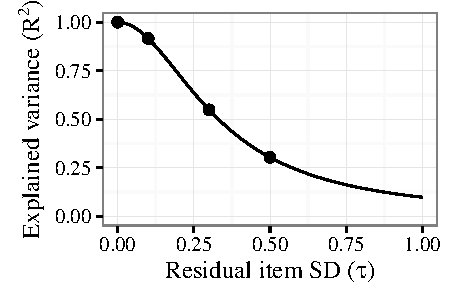
\includegraphics[height=3in, trim = 1mm 1mm 1mm 1mm, clip=true]
		{chapter_2/figs/rsq_vs_tau.pdf}
	\caption{$R^2$ versus $\tau$ for the simulations. The points indicate generating values of $\tau$.}
	\label{fig:rsq-vs-tau}
\end{figure}

In summary, three factors are varied between simulation conditions in a crossed design: $\tau$ (and by extention, $R^2$), $I$, and $P$. All other elements are fixed across conditions. Because cross-validation features prominently in this chapter, multiple datasets are simulated within each replication. A ``training'' dataset is created as described above, and along with it three ``test'' datasets are formed: one representing a sample with new items (corresponding to new draws of $\epsilon_i$), one representing a sample with new persons (new draws of $\zeta_p$), and the last representing a sample with both new items and new persons.


\subsection{Models}

Three models, differing only in specification of $\delta_i$, are fit. Model 1 includes only the ``main effects'' for the item covariates:
\begin{equation}
\delta_i^{(1)} = x_{1i}\beta_1 + x_{2i}\beta_2 + x_{3i}\beta_3 + x_{4i}\beta_4
.\end{equation}
Model 2 adds an interaction:
\begin{equation}
\delta_i^{(2)} = x_{1i}\beta_1 + x_{2i}\beta_2 + x_{3i}\beta_3 + x_{4i}\beta_4
+ x_{2i}x_{3i}\beta_5
.\end{equation}
Model 3 adds an additional, extraneous interaction:
\begin{equation}
\delta_i^{(3)} = x_{1i}\beta_1 + x_{2i}\beta_2 + x_{3i}\beta_3 + x_{4i}\beta_4
+ x_{2i}x_{3i}\beta_5 + x_{3i}x_{4i}\beta_6
.\end{equation}
None of the analysis models includes the residual $\epsilon_i$. Each analysis model models ability as in Equations~\ref{eq:theta} and \ref{eq:zeta}. %When $\tau = 0$ is used to generate the data, Model 2 is the true model. Otherwise, none of three match the data generating model.


\section{Naive cross-validation methods}

One naive approach to model selection is the use of significance testing for parameters. In order to select among the three analysis models, a researcher may fit Model~2 and make a judgment based on the p-value for $\beta_5$, the parameter associated with the interaction. If non-significant, the researcher may select Model~1. Otherwise, the researcher may fit Model~3. If the additional interaction ($\beta_6$) is significant, Model~3 would be selected. Otherwise, Model~2 would be selected. This is a forward stepwise procedure.

%Figure~\ref{fig:pcheck-bar} presents the proportion of times each model was selected across conditions (combination of $I$, $P$, and $\tau$) when selection is performed via p-values. Within each condition, 200 replications are performed. This method works well when $\tau$ is small but poorly otherwise, and this trend is similar for all combinations of $P$ and $I$. 
This method works well when $\tau$ is small but poorly otherwise.
When $\tau = 0$, Model~2 matches the data generating model exactly, and Models~1 and 3 are close. The result is that the correlated nature of responses within an item cluster are appropriately accounted for, yielding correct standard errors for $\mathbf{\beta}$. The preceding is approximately true for small values of $\tau$ like $\tau = .1$. However, with greater values of $\tau$, the analysis models fail to account for the within-cluster dependency, resulting in standard errors that are too low. This shortcoming leads to Model~3 being selected the majority of the time when $\tau$ takes medium to large values.
\comment{Add back in results supporting this or remove.}

%\begin{figure}[htbp]
%	\centering
%	\includegraphics[height=3.5in, trim = 1mm 1mm 1mm 1mm, clip=true]
%	{chapter_2/figs/p_pcheck.pdf}
%	\caption{Proportion of times each model was selected using significance tests.}
%	\label{fig:pcheck-bar}
%\end{figure}

Adding item residuals $\epsilon_i$ to the analysis models would provide correct standard errors and p-values. Such a model is prohibitively difficult to fit without resorting to Monte Carlo methods, though. Further, in practical application there may be many more than three models under consideration, which brings up complexities around multiple hypothesis testing. For this reason an appealing alternative is AIC, defined as
\begin{equation} \label{eq:aic}
	\mathrm{AIC} = \mathrm{deviance} + 2k
,\end{equation}
where $k$ is the number of model parameters. The model with the lowest value of AIC is selected. The results of using AIC with the simulated datasets are presented in Figure~\ref{fig:select-aic}. 
%These results follow similar patterns as for selection by p-values, though a bit worse.

\begin{figure}[tbp]
	\centering
	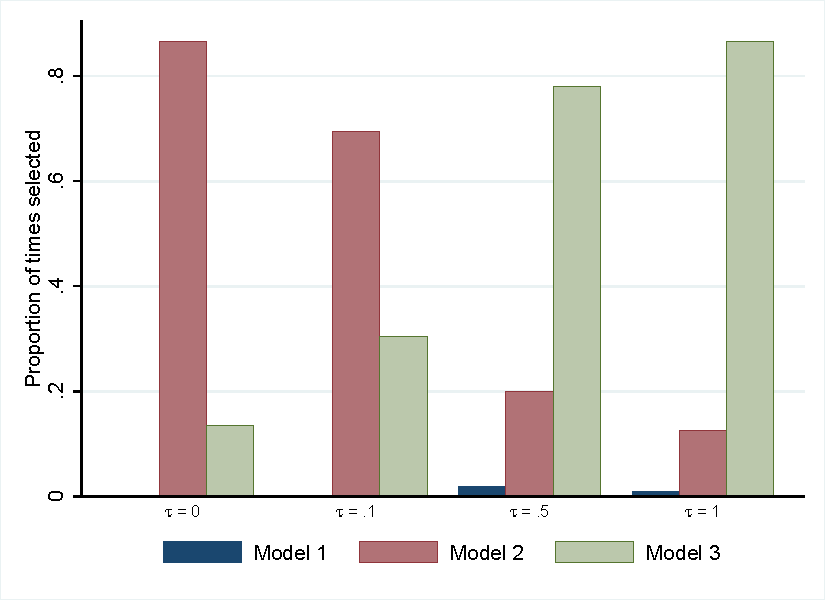
\includegraphics[height=3in, trim = 1mm 1mm 1mm 1mm, clip=true]
		{chapter_2/figs/select_aic.pdf}
	\caption{Proportion of times each model was selected using AIC.}
	\label{fig:select-aic}
\end{figure}

AIC is an approximation for holdout cross-validation, in which a model is estimated using a ``training'' dataset and then evaluated on a ``test'' dataset. In this instance, AIC approximates the deviance that would result from applying the trained model to a test dataset consisting of new persons and the same items. \comment{Explain why, from chapter 1 or cite papers.} $k$ in Equation~\ref{eq:aic} may be viewed as an adjustment to the deviance of the model fit to the training data owing to uncertainty in the parameter estimates. 

The correct values for $k$ may be estimated from the simulation by subtracting the deviance from the model fit to the training data from the fit to test data consisting of new persons responding to the same items. This is presented in Figure~\ref{fig:k-new-persons}. The empirical estimates for $k$ are similar to those given by AIC (\aic[and]) with some variation across values for $\tau$. Importantly, the difference between models is consistent across values for $\tau$ and with AIC.

\begin{figure}[tbp]
	\centering
	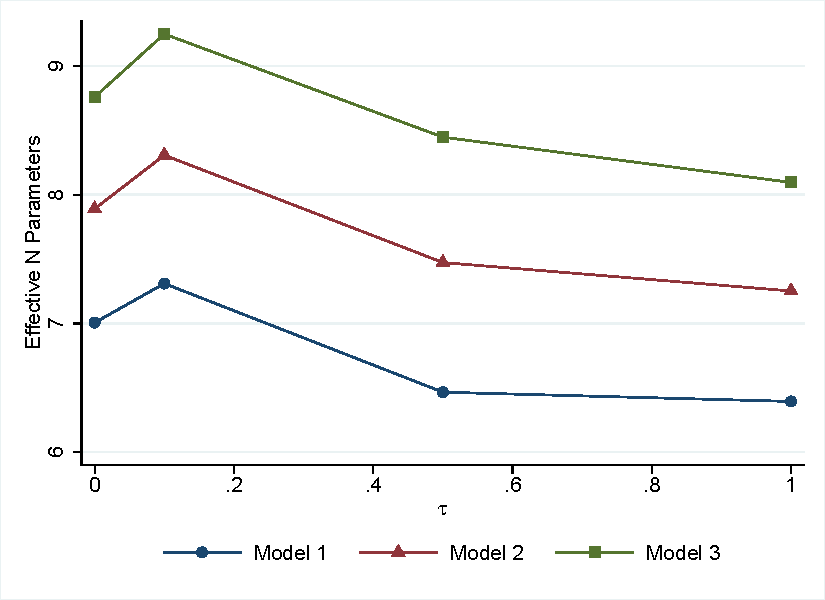
\includegraphics[height=3in, trim = 1mm 1mm 1mm 1mm, clip=true]
	{chapter_2/figs/p_newpersons.pdf}
	\caption{Estimated effective number of parameters for models fit to test data consisting of new persons responding to the same items.}
	\label{fig:k-new-persons}
\end{figure}

In short, AIC performs poorly for model selection in this instance even though it accurately estimates the out-of-sample deviance. Further, cross-validation with new persons also performs poorly, as depicted in Figure~\ref{fig:select-new-persons}. Lastly, BIC performs somewhat better but has the same problem, as shown in Figure~\ref{fig:select-bic}.

\begin{figure}[tbp]
	\centering
	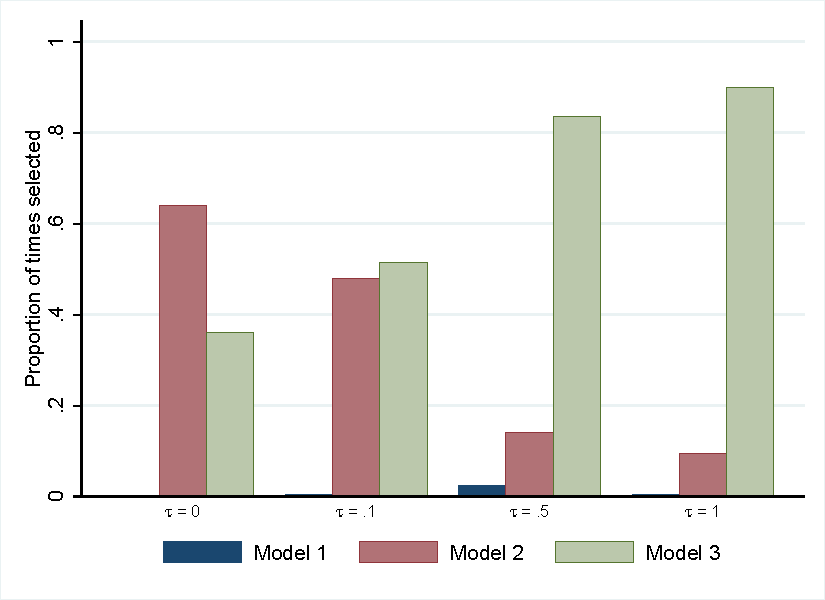
\includegraphics[height=3in, trim = 1mm 1mm 1mm 1mm, clip=true]
	{chapter_2/figs/select_newpersons.pdf}
	\caption{Proportion of times each model was selected using cross-validation with new perons.}
	\label{fig:select-new-persons}
\end{figure}

\begin{figure}[tbp]
	\centering
	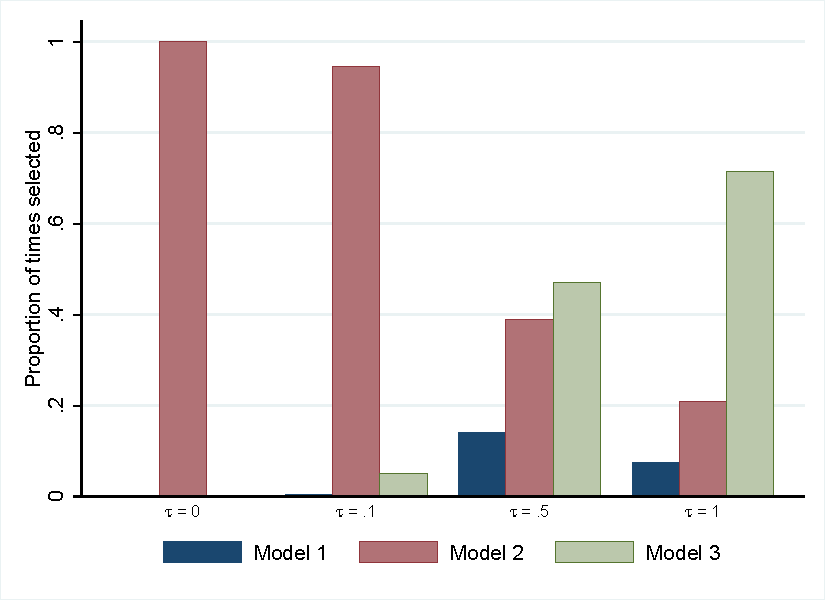
\includegraphics[height=3in, trim = 1mm 1mm 1mm 1mm, clip=true]
	{chapter_2/figs/select_bic.pdf}
	\caption{Proportion of times each model was selected using BIC.}
	\label{fig:select-bic}
\end{figure}


\section{Holdout cross-validation for item predictors}

If the focus of model selection is the choice of item predictors, cross-validation schemes based on test data with the same items are wrongheaded. A useful approach instead is to consider how the item predictors will fare for a new set of items constructed from the same item design. To this end, the analysis models are fit to a training dataset and then evaluated on a holdout dataset representing the same persons and new items. Figure~\ref{fig:select-newitems} provides the proportion of times each model was selected using this scheme. 
%Across all conditions, Model~2 is selected the majority of times. For $I=32$ items, larger values of $\tau$ are associated with a lower selection proportion for Model~2, while this trend is mitigated when $I=128$.

\begin{figure}[tbp]
	\centering
	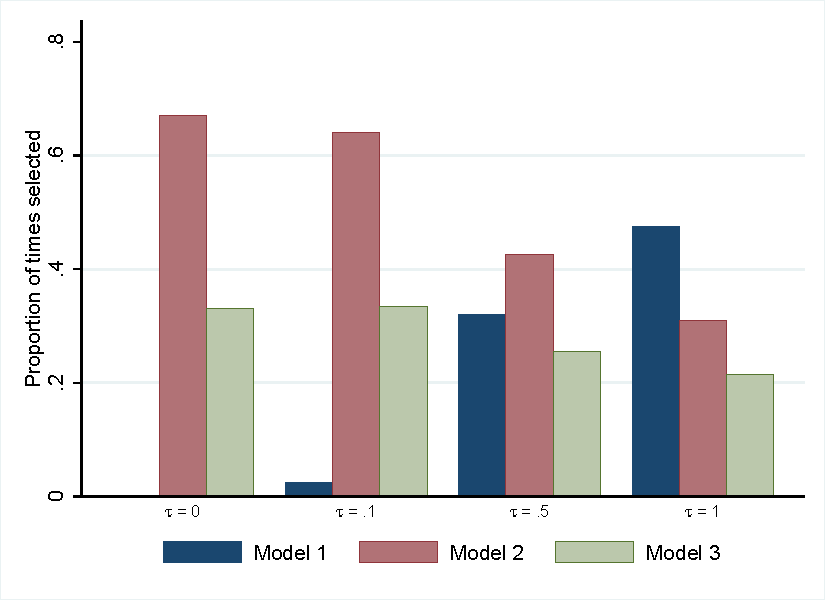
\includegraphics[height=3.5in, trim = 1mm 1mm 1mm 1mm, clip=true]
		{chapter_2/figs/select_newitems.pdf}
	\caption{Proportion of times each model was selected using holdout cross-validation with holdout data consisting of the same persons and new items.}
	\label{fig:select-newitems}
\end{figure}


\section{Cross-validation with a fixed-persons random-items model.}

A variation on the three models is considered in which the persons are modeled as fixed effects and the items as random effects. The fixed part of the models include the item predictors and and indicator variable for each sum score. Person covariates are omitted. In these ``inverted'' models, the items are regarded as exchangeable rather than the persons. It is posited that AIC for the inverted models would perform correctly for cross-validation inferences that involve new items.

Figure~\ref{fig:k-new-items} provides the estimated effective number of parameters for the models based on the simulations. As may be seen, the values are low in comparison with the count of parameters (\aicitem[and]) and dependent on $\tau$. Figure~\ref{fig:select-aicitem} shows the proportion of times each inverted model was selected using AIC.

\begin{figure}[tbp]
	\centering
	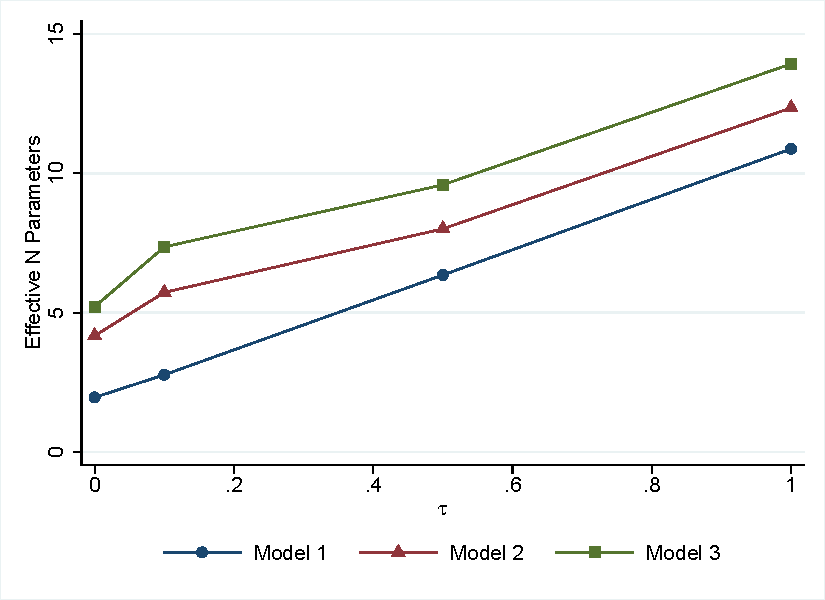
\includegraphics[height=3in, trim = 1mm 1mm 1mm 1mm, clip=true]
	{chapter_2/figs/p_newitems.pdf}
	\caption{Estimated effective number of parameters for models fit to test data consisting of the same persons responding to new items.}
	\label{fig:k-new-items}
\end{figure}

\begin{figure}[tbp]
	\centering
	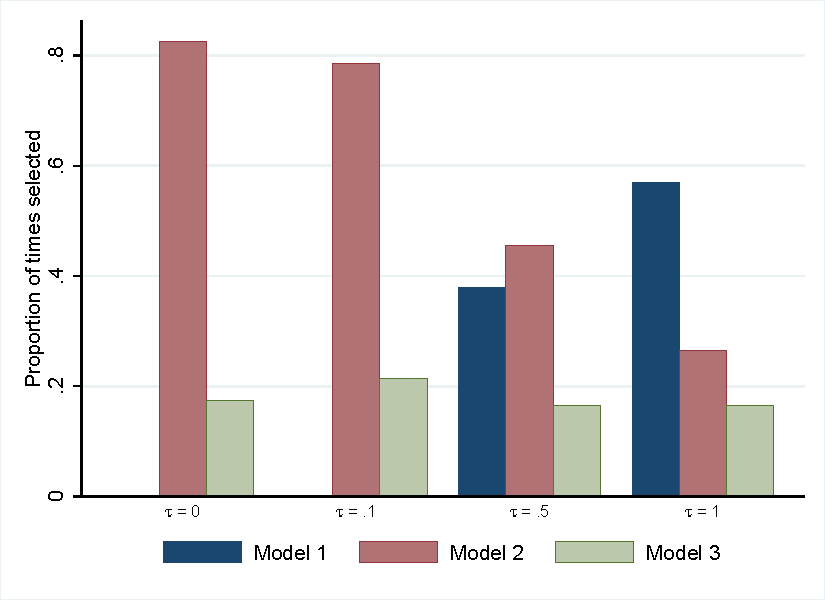
\includegraphics[height=3.5in, trim = 1mm 1mm 1mm 1mm, clip=true]
	{chapter_2/figs/select_aic2.pdf}
	\caption{Proportion of times each model was selected using AIC with the ``inverted'' models.}
	\label{fig:select-aicitem}
\end{figure}


\section{Discussion}

\comment{Find papers on choosing between LLTMS.}

\comment{(1) K-fold CV. (2) Consider a linear model to parallel holdout CV with new items. Possible to get marginal likelihood with linear model? (3) Show that AIC works with ``De Boeck'' version of model. (4) Consider extending topic to include linear crossed mixed-effects models.}

%\bibliographystyle{apacite}
%\bibliography{../../Documents/References/references}

\end{document}




\newpage
\chapter{Bayesian cross-validation with the doubly explanatory model}
\chaptermark{Bayesian cross-validation}
The final chapter takes advantage of the Bayesian framework to implement effective (I expect) methods for the selection of item covariates. 
With MCMC methods, the doubly explanatory model may be estimated maintaining both the person and item residuals, and recently developed Bayesian cross-validation approximations are readily calculated from the conditional likelihood given these residuals after MCMC simulation. 
However, these approximations correspond to a cross-validation scheme in which holdout data include new responses from the same persons and same items. 
For inferences requiring, for example, cross-validation over items, I will show that a marginal variation of these approximations is superior (I expect).
The methods are first introduced for a simpler model and are then extend to the doubly explanatory model.


\section{WAIC and Bayesian LOO}

As a simple example, consider a hierarchical model (not cross-clustered) in which a response $y_{jk}$ has a likelihood, 
$p(y_{jk} | \theta_k)$, 
that is conditional on a cluster-specific parameter $\theta_k$. This parameter has a hierarchical prior,
$\theta_k \sim \mathrm{N}(0, \psi)$, and in turn the variance has as a prior
$\psi \sim \mathrm{log~N}(0, 1)$, an arbitrary choice. For Bayesian cross-validation, the pointwise predictive density is defined as the conditional likelihood integrated over the posterior distributions of all parameters. For the simple example, this quantity is
\begin{equation} 
	\mathrm{PD}_{jk} = 
	\iint
		p(y_{jk} | \theta_k)
		p(\theta_k | D, \psi)
		p(\psi | D)
	~d \theta_k d \psi
,\end{equation}
where $D$ represents all the data, in this case merely the complete response vector.
The log of $\mathrm{PD}_{jk}$ may be summed across observations to calculate a full data log-likelihood.
In an MCMC simulation with $S$ posterior draws, this quantity may be evaluated at each posterior draw $s$ as
\begin{equation} 
	\mathrm{PD}_{jk}^{(s)} = 
	p(y_{jk} | \theta_k^{(s)})
	p(\theta_k^{(s)} | D, \psi^{(s)})
	p(\psi^{(s)} | D)
,\end{equation}
where $\theta_k^{(s)}$ represents the posterior draw of $\theta_k$ at MCMC iteration $s$ and likewise for $\psi^{(s)}$.
$\mathrm{PD}_{jk}^{(s)}$ may be aggregated across draws to estimate the posterior distribution of $\mathrm{PD}_{jk}$. Usually this topic is discussed in terms of the \emph{log} pointwise predictive density (for example, \cite{gelman2014understanding}), but breaking from this norm simplifies some notation that follows.

Keeping with the simple example, WAIC \parencite{watanabe2010asymptotic}, a Bayesian information criteria, is defined as
\begin{equation} \label{eq:waic}
	\mathrm{WAIC} = 
		\sum_{k=1}^K \sum_{j=1}^J \log  
			\left (\frac{1}{S} \sum_{s=1}^{S} \mathrm{PD}_{jk}^{(s)} \right ) -
		\sum_{k=1}^K \sum_{j=1}^J V_{s=1}^{S} 
			\left ( \log \mathrm{PD}_{jk}^{(s)} \right )
\end{equation}
where $V_{s=1}^{S}$ represents the sample variance.
Like other information criteria, it has the form of log likelihood minus a penalty term. The penalty term for WAIC is estimated from the variances of the log pointwise predictive densities. Although the equation shows separate summations over $j$ and $k$, the summations are only a means of aggregating over the full data and do not really reflect the nested nature of the data. WAIC bears some similarity to DIC \parencite{Spiegelhalter2002} but is more stable \parencite{vehtari2015efficient}.

Bayesian LOO is an estimate of the $\mathrm{PD}_{jk}$ that would result from leave one out cross-validation. 
\textcite{gelfand1992model} propose estimating this quantity using importance sampling, and \textcite{vehtari2015efficient} propose smoothing the distribution of importance weights by fitting a generalized Pareto distribution to the upper tail of the weights.


\section{Marginal forms of WAIC and Bayesian LOO}

A limitation of cross-validation approximations relying on $\mathrm{PD}_{jk}^{(s)}$ is that they imply a cross-validation scheme in which the same clusters are represented in the holdout dataset. For inferences regarding cross-validation with new clusters, I propose a marginal predictive pointwise density:
\begin{equation} \label{eq:mpd-easy}
	\mathrm{MPD}_{k}^{(s)} = 
	%\log 
	\left (
		\left [ \int
			p(\check \theta | \psi^{(s)})
			\prod_{j} p(y_{jk} | \check \theta)
			~d \check \theta
    \right ]
		p(\psi^{(s)} | D)
	\right )
.\end{equation}
The accent is placed on $\check \theta$ to indicate that it is not 
drawn from its posterior distribution but from its ``prior'' distribution, given the posterior draw of $\psi^{(s)}$. 
In short, the bracketed quantity is the joint likelihood of cluster $k$ integrated over $p(\check \theta | \psi^{(s)})$, which is not directly influenced by data from cluster $k$.
This is similar to marginalizing over ``random effects'' in frequentist mixed models, except here it occurs at every posterior draw $s$. $\mathrm{MPD}_{k}^{(s)}$ may be used in place of $\mathrm{PD}_{jk}$ for calculating WAIC and Bayesian LOO when cross-validation with clusters is needed. The integration in Equation~\ref{eq:mpd-easy} has a closed form for linear models, and for models with non-linear link functions I proposed estimating it with adaptive quadrature \parencite{naylor1982applications}, which has been shown to work well for models with discrete outcomes and large clusters \parencite{rabe2005maximum}.

Returning now to the context of the doubly explanatory model, the pointwise predictive density is
\begin{equation} \label{eq:eirm-lpd}
	\mathrm{PD}_{ip}^{(s)} = 
		p(y_{ip} | \zeta_p^{(s)}, \epsilon_i^{(s)})
		p(\zeta_p^{(s)} | D, \sigma^{(s)})
		p(\epsilon_i^{(s)} | D, \tau^{(s)}) 
		p(\sigma^{(s)}, \tau^{(s)} | D)
,\end{equation}
where $D$ again represents all the data, in this case including all responses in $y$, the person covariate matrix $W$, and the item covariate matrix $X$. For models for cross-clustered data, including the doubly explanatory model, I propose calculating the marginal pointwise predictive density in such a way as to be marginal in regard to one set of clusters but not the other. For cross-validation over persons,
\begin{equation}
	\mathrm{MPD}_p^{(s)} = 
		\left [ \int
			p(\check \zeta | \sigma^{(s)})
			\prod_{i=1}^I	p(y_{ip} | \check \zeta, \epsilon_i^{(s)})
			~d \check \zeta 
		\right ]
		p(\epsilon^{(s)} | D, \tau^{(s)}) 
		p(\sigma^{(s)}, \tau^{(s)} | D)
\end{equation}
is appropriate. Here it is assumed that the same items would be administered to new person, and so the quantity is marginal only in regards to persons. On the other hand,
\begin{equation}
	\mathrm{MPD}_i^{(s)} = 
		\left [ \int
			p(\check \epsilon | \tau^{(s)})
			\prod_{p=1}^P	p(y_{ip} | \zeta^{(s)}, \check \epsilon_i)
			~d \check \epsilon 
		\right ]
		p(\zeta^{(s)} | D, \sigma^{(s)}) 
		p(\sigma^{(s)}, \tau^{(s)} | D)
,\end{equation}
which is marginal in regards to items, may be used for cross-validation over items.


\section{Simulation study 1: Linear responses}

I will conduct a simulation study, similar to those in Chapter~2, that evaluates the success that standard and marginal versions of WAIC and Bayesian LOO exhibit in selecting the correct model among models with differing item covariates. I will first use a version of the doubly descriptive model that is modified to have a continuous response variable. Doing so will allow me simultaneously study (1) how WAIC and Bayesian LOO perform when the likelihoods need not be approximated and (2) the accuracy of adaptive quadrature as compared against the exact likelihoods.

Owing to the relative slowness of MCMC simulation, this simulation study will involve fewer conditions as compared to those in Chapter~2 and may not incorporate holdout cross-validation. Also, if simulation study~2 (below) is highly successful, simulation study~1 may be abbreviated or omitted. Preliminary results indicate that adaptive quadrature works very well in simpler random intercept models. Also for the random intercept model, I find that the marginal forms of WAIC and Bayesian LOO are successful in choosing the generating model in a high proportion of replications.


\section{Simulation study 2: Categorical responses}

The second simulation study will use the unmodified doubly explanatory model. It will track the success that standard and marginal versions of WAIC and Bayesian LOO exhibit in selecting the correct model among models with differing item covariates. It will be very similar to simulation study~1, with the only difference being the binary response variable and the use of adaptive quadrature.


% \appendix
% \chapter{More Monticello Candidates}

\printbibliography

\end{document}
